\documentclass[tikz]{standalone}
\usepackage{amsmath}
\usepackage{times}
\usepackage{txfonts}

\usetikzlibrary{arrows}
\usetikzlibrary{shapes.geometric}
\usetikzlibrary{intersections}
\usetikzlibrary{math}
\usetikzlibrary{positioning}
\usetikzlibrary{arrows.meta}
\usetikzlibrary{shapes.misc}
\usetikzlibrary{calc}

\begin{document}
	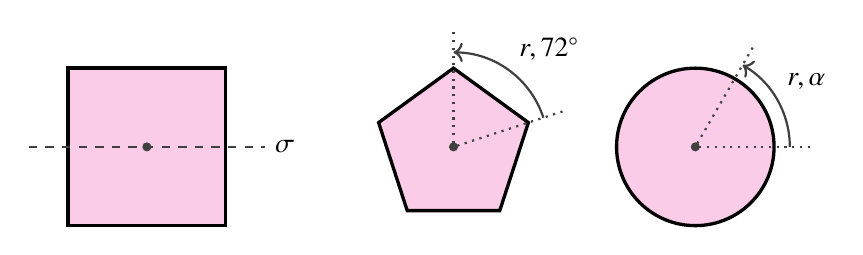
\begin{tikzpicture}[
			node distance = 2cm,
			shapetheme/.style = {
				very thick, draw = black, fill = magenta!20!white,
				minimum size = 2cm,
			},
			line/.style = {thick, draw = darkgray},
			axis/.style = {line, dashed},
			dot/.style = {
				circle, draw = darkgray, fill = darkgray,
				minimum size = 1mm, inner sep = 0, outer sep = 0,
			},
		]

		\node[
			shapetheme, rectangle
		] (R) {};
		\node[dot] at (R) {};
		\draw[axis] (R) ++(-1.5, 0) to ++(3, 0) node[right] {\(\sigma\)};

		\node[
			shapetheme,
			regular polygon,
			regular polygon sides = 5,
			right = of R,
		] (Ps) {};
		\node[dot] (P) at (Ps) {};
		\draw[line, dotted] (P) to ++(18:1.5);
		\draw[line, dotted] (P) to ++(90:1.5);
		\draw[line, ->] (P) ++(18:1.2) 
			arc (18:90:1.2) node[midway, above right] {\(r, 72^\circ\)};

		\node[
			shapetheme,
			circle, right = of P
		] (Cs) {};
		\node[dot] (C) at (Cs) {};
		\draw[line, dotted] (C) to ++(1.5,0);
		\draw[line, dotted] (C) to ++(60:1.5);
		\draw[line, ->] (C) ++(1.2,0)
			arc (0:60:1.2) node[midway, above right] {\(r, \alpha\)};

	\end{tikzpicture}
\end{document}
